\scanpage{53}
\mspage{6}
L'isom. canonique déduit de l'inclusion.

On a de plus des isomorphismes canoniques
\[
(30)\quad\left\{\begin{aligned}
\varphi_{i\varepsilon}&:\Pi_\omega\longrightarrow\Pi_i\qquad\text{défini par }c_i^\varepsilon:P_\varepsilon\longrightarrow Q_i\\
\varphi_{\varepsilon i}&:\Pi_i\longrightarrow\Pi_\omega\qquad\text{---}\qquad(c_i^\varepsilon)^{-1}:Q_i\longrightarrow P_\varepsilon
\end{aligned}\right.
\]
\margin{\uline{NB} on a $\varphi_{i\varepsilon}=\varphi_{Q_i,\varepsilon}$, $\varphi_{\varepsilon i}=\varphi_{P_\varepsilon,i}$.}
Par ces isom., les $\Pi_\varepsilon,\Pi_i$ sont reliés de façon transitive, mais bien entendu pas par un syst. transitif d'isomorphismes -- au contraire, les autom. d'un des groupes $\Pi_\varepsilon,\Pi_i$ obtenus en composant des isoms 30, suivant des chemins fermés sur le graphe
\figure{
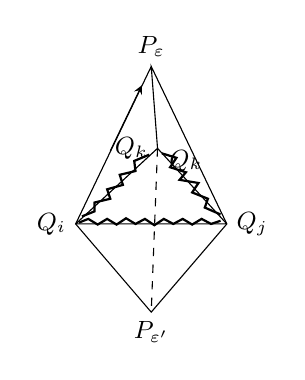
\begin{tikzpicture}[x=.8cm,y=.8cm,>=stealth,every node/.style={font=\small}]
\coordinate (P) at (0,2.5);\coordinate (M) at (0,-1.4);\coordinate (I) at (-1.2,0);\coordinate (J) at (1.2,0);\coordinate (K) at (.1,1.2);
\draw (P)--(I)--(M)--(J)--(P)--(K);
\draw[dashed] (K)--(M);
\draw[->] (-.65,1.16)--(-.15,2.2);
\draw (I)--(J) (I)--(K)--(J);
\draw[thick] (-1.15,.02)--(-1,.08)--(-.85,-.01)--(-.7,.08)--(-.55,-.01)--(-.4,.09)--(-.25,0)--(-.1,.08)--(.05,-.02)--(.2,.08)--(.35,0)--(.5,.08)--(.65,-.01)--(.8,.08)--(.95,0)--(1.1,.05);
\draw[thick] (-1.1,.12)--(-.9,.2)--(-.9,.34)--(-.65,.4)--(-.7,.55)--(-.45,.62)--(-.5,.78)--(-.25,.84)--(-.27,1)--(-.03,1.1);
\draw[thick] (.17,1.12)--(.4,1.05)--(.3,.9)--(.55,.82)--(.45,.7)--(.75,.65)--(.65,.5)--(.9,.4)--(.85,.26)--(1.1,.15);
\node[above] at (P) {$P_\varepsilon$};\node[below] at (M) {$P_{\varepsilon'}$};\node[left] at (I) {$Q_i$};\node[right] at (J) {$Q_j$};\node[left] at (K) {$Q_k$};
\node at (.55,1) {$\deleted{\unsure{Q_k}}$};
\end{tikzpicture}
}
sont \uline{tous} les autom. intérieurs !

Les $\Pi_1(\Sigma^*,\text{en }-)$ en les $P_\varepsilon,Q_i$ étant \unsure{canonifiés|canonisés} comme les $\Pi_\varepsilon,\Pi_i$, il reste à ``repérer'' les $\Pi_1$ en les autres sommets marqués jusqu'à maintenant. Les choix naturels sont par
\deleted{$\unsure{\varphi_\varepsilon}\ \Pi_\varepsilon\quad\unsure{\varphi_i}\ \Pi_i\longrightarrow$}
\margin{52}
